 \question{Berechnen Sie die Antwort des gedämpften Einmassenschwingers aus Aufgabe 2 TODO fix reference
(letzte Übung) auf das Sägezahnsignal $(T = \SI{1}{\second}, u_{max} = - u_{min} = \SI{0.1}{\meter})$,
welches durch eine Fourierreihe bis $N = 2$ approximiert werden soll. Als
Anfangsbedingungen gelten: $u(-T/2) = \SI{0}{\meter}, \hat{u}(-T/2) = \SI{0}{\meter\per\second}
$.}

\begin{minipage}[c]{.49\linewidth}
 \begin{align*}
     a(t) = \frac{2a_{max}}{T}t -nT \\
     nT - \frac{T}{2} < t \leq nT + \frac{T}{2}
 \end{align*}
 \end{minipage}
     
     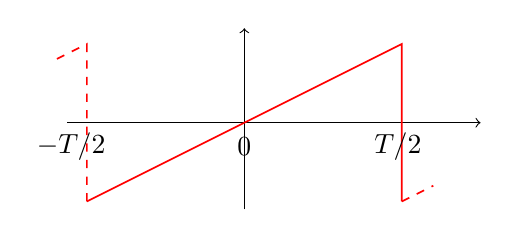
\begin{tikzpicture}[baseline=0mm] 
\draw[->] (-2.25, 0) -- (3, 0);
\draw[->] ( 0,-1.1) -- (0, 1.2);
\draw[semithick,red] (-2,-1) -- ( 2, 1) -- (2,-1);
\draw[semithick,red, dashed] (-2,-1) -- (-2, 1) -- (-2.4, 0.8);
\draw[semithick,red, dashed] ( 2,-1) -- ( 2.4,-0.8);
\draw (-2.2,-0.3) node {$-T/2$};
\draw ( 0,-0.3) node {$0$};
\draw ( 1.95,-0.3) node {$T/2$};
\end{tikzpicture}


\begin{solution}
\begin{minipage}[c]{.49\linewidth}
 \begin{align*}
     a(t) &= ct \\
     c &= \frac{2a_{max}}{T} \\
     \tilde{w}_k &= \frac{2\pi k}{T}
 \end{align*}
\end{minipage}

 \textbf{\raggedright Darstellung der Anregung als Fourierreihe ($N=2$)}

\vspace{1em}

\begin{align*}
    \intertext{\flushleft Benötigte Integrale:}
    \int x \sin(ax) \dd{x} &= \frac{\sin(ax) - x \cos(ax)}{a} \\
    \int x \cos(ax) \dd{x} &= \frac{\cos(ax) + x \sin(ax)}{a}
\end{align*}

\dotfill

\begin{align*}
    A_0 &=  \frac{2}{T} \int\limits_{-\frac{T}{2}}^{\frac{T}{2}} a(t)\dd{t} = \frac{2}{T} \int\limits_{-\frac{T}{2}}^{\frac{T}{2}} ct \dd{t} = \frac{2}{T} \,\Big|\, \frac{c}{2}t^2\,\Big|_{t = -\frac{T}{2}}^{\frac{T}{2}} = \uuline{0}\\
    A_k &= \frac{2}{T} \int\limits_{-\frac{T}{2}}^{\frac{T}{2}} a(t) \cos(\overbrace{\frac{2\pi k}{T}}^{\tilde{w}_k}t)\dd{t} = \frac{2}{T} \int\limits_{-\frac{T}{2}}^{\frac{T}{2}} ct \cos(\tilde{w}_k t) \dd{t} \\
    &= \frac{2}{T} \,\Big|\,\frac{c}{\tilde{w}_k} (\cos(\tilde{w}_k t) + t \sin(\tilde{w}_k t))\,\Big|_{t = -\frac{T}{2}}^{\frac{T}{2}} = \uuline{0}
\end{align*}


\begin{minipage}[t]{.49\linewidth}

      $\cos(\tilde{w}_k t)$\\

      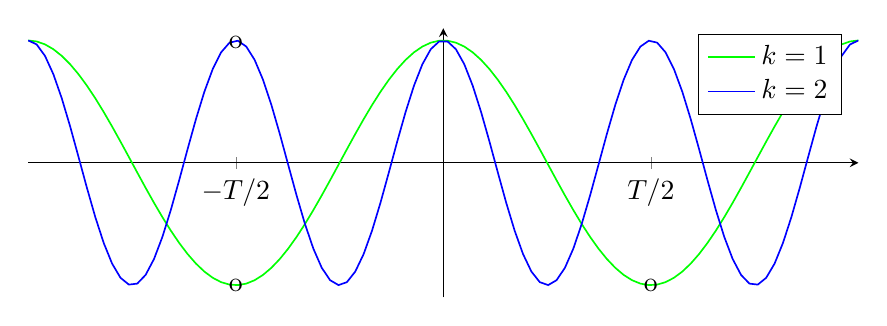
\begin{tikzpicture}
    \begin{axis}[
        width = \linewidth,
        height = 5cm,
        axis x line=center,
        axis y line=middle,
        samples=100,
        ymin=-1.1, ymax=1.1,
        xmin=-pi, xmax=pi,
        ytick=\empty,
        xtick={-pi/2,pi/2},
        xticklabels={$-T/2$,$T/2$}
        ]
        \addplot [semithick, green, domain=-pi:pi] {cos(2*deg(x))};
        \addlegendentry{$k=1$};
        \addplot [semithick, blue, domain=-pi:pi] {cos(4*deg(x))};
        \addlegendentry{$k=2$};
        \draw (axis cs: -1.57,0.98) node {o};
        \draw (axis cs: -1.57,-1) node {o};
        \draw (axis cs:  1.57,-1) node {o};
    \end{axis}
\end{tikzpicture}

\end{minipage}
\begin{minipage}[t]{.49\linewidth}

    $\sin(\tilde{w}_k t)$\\

    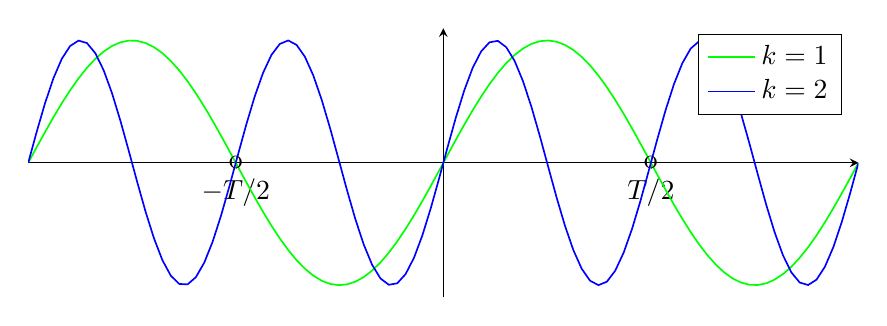
\begin{tikzpicture}
    \begin{axis}[
        width = \linewidth,
        height = 5cm,
        axis x line=center,
        axis y line=middle,
        samples=100,
        ymin=-1.1, ymax=1.1,
        xmin=-pi, xmax=pi,
        ytick = \empty,
        xtick={-pi/2,pi/2},
        xticklabels={$-T/2$,$T/2$}
        %legend style={draw=none}
        ]
        \addplot [semithick, green, domain=-pi:pi] {sin(2*deg(x))};
        \addlegendentry{$k=1$};
        \addplot [semithick, blue, domain=-pi:pi] {sin(4*deg(x))};
        \addlegendentry{$k=2$};
        \draw (axis cs: -1.57,0) node {o};
        \draw (axis cs:  1.57,0) node {o};
    \end{axis}
\end{tikzpicture}

\end{minipage}
\vspace{1em}

\begin{align*}
     B_k &= \frac{2}{T} \int\limits_{-\frac{2}{T}}^{\frac{2}{T}} ct \sin(\tilde{w}_k t) \dd{t} = \frac{2}{T}\,\Big|\, \frac{c}{\tilde{w}_k}(\sin(\tilde{w}_k t)-t\cos(\tilde{w}_k t))\,\Big|_{t={-\frac{2}{T}}}^{t=\frac{2}{t}} \\
     &= \frac{-2c}{\tilde{w}_k} \cos(\tilde{w}_k\frac{T}{2}) =
     \left\{
     \begin{array}{lll}
     \cfrac{2c}{\tilde{w}_k} & &k = 1,3,5,\dots\\[1em]
     -\cfrac{2c}{\tilde{w}_k} & &k = 2,4,6,\dots
     \end{array}\right.
\end{align*}

\begin{align*}
     \begin{array}{lcl}
        a = \overbrace{B_1\sin(\tilde{w}_1 t)}^{a_1(t)} + \overbrace{B_1\sin(\tilde{w}_2 t)}^{a_2(t)} & \rightsquigarrow & u_p(t) = u_{p1}(t) + u_{p2}(t) \\[1em]
        B_1 = \cfrac{4a_{max}\cancel{T}}{2\pi\cancel{T}} \qquad \tilde{w}_1 = \cfrac{2\pi}{T} && u_{p1}^{(t)} = u_{C1} \cos(\tilde{w}_k t) + u_{S1} \sin(\tilde{w}_1 t) \\[1em]
        B_2 = \cfrac{4a_{max}}{4\pi} \qquad \tilde{w}_2 = \cfrac{4\pi}{T}&& \underbrace{u_{p2}^{(t)} = u_{C2} \cos(\tilde{w}_k t) + u_{S2} \sin(\tilde{w}_2 t)} \\
        &&\text{Partikuläre Lösung - siehe Übung}\\
        &&\text{harmonisch erregter Einmassenschwinger}
    \end{array}
\end{align*}\\[2em]

\textbf{Anpassung der Gesamtlösung an die Anfangsbedingungen}
    
    Die Gesamtlösung setzt sich additiv aus der Lösung der homogenen Gleichung und der bereits bestimmten Partikulärlösung zusammen
    \begin{align*}
        u(t) &= C_1\cos(\omega_1 t)e^{-\delta t} + C_2 \sin(\omega_1 t)e^{-\delta t} + u_p(t),\\
        \dot{u}(t) &= -C_1 \exp(-\delta t) \cdot (\omega_1 \sin(\omega_1 t) + \delta \cos(\omega_1 t)) + C_2 \exp(-\delta t) \cdot (\cos(\omega_1 t) + \sin(\omega_1 t)) + \dot{u_p}(t).
    \end{align*}
    Mit den Anfangsbedingungen
    \begin{align*}
        u(t_0) &= u_0 \\
        \dot{u}(t_0) &= \dot{u}_0
    \end{align*}
    liegen zwei Gleichungen mit zwei Unbekannten vor
    \begin{align*}
    \begin{bmatrix}
        A_{11} & A_{12}\\
        A_{21} & A_{22}
    \end{bmatrix}
    \begin{bmatrix}
        C_1 \\
        C_2
    \end{bmatrix}
    &=
    \begin{bmatrix}
    b_1 \\
    b_2
    \end{bmatrix} \\
    \intertext{mit}
        A_{11}&= -\omega_1 \sin(\omega_1 t) \exp(-\delta t),\\
        A_{12}&= - \delta \cos(\omega_1 t) \exp(-\delta t),\\
        A_{21}&= \cos(\omega_1 t) \exp(-\delta t),\\
        A_{22}&= \sin(\omega_1 t) \exp(-\delta t),\\
        b_{1}&= -u_{C_1} \tilde{\omega_k} \sin(\tilde{\omega_k}t) + u_{S_1} \tilde{\omega_1} \cos(\tilde{\omega_1}t),\\
        b_{2}&= -u_{C_2} \tilde{\omega_k} \sin(\tilde{\omega_k}t) + u_{S_2} \tilde{\omega_2} \cos(\tilde{\omega_2}t).
    \end{align*}

    \begin{align*}
        T_a &= \SI{9}{\second} \\
        k &=  \SI{10}{\newton \per \second} \\
        c &= \SI{1}{\newton \second \per \meter} \\
        a_{C_1} &= 0 \\
        a_{S_1} &= 1 \\
        \omega &= \frac{2 \pi}{T_a} &&= 0.698 \\
        \omega_0 &= \sqrt{\frac{k}{m}} &&= 1.826\\
        \zeta &= \frac{c}{2 \sqrt{km}} &&= 0.091\\
        \eta &= \frac{\omega}{\omega_0} &&= 0.382\\
        V &= \frac{1.0}{\sqrt{(1-\eta^2)^2 - (2 \zeta \eta)^2}} &&= 1.608\\
        u_{C_1}  &= V^2 ((1-\eta^2) a_{c_1} - 2 \zeta \eta a_{s_1}) &&= -0.095 \\ 
        u_{S_1} &= V^2 ((1-\eta^2) a_{s_1} - 2 \zeta \eta a_{c_1}) &&= 1.163 \\  
        u_{p_1}(t) &= -0.095 \cos(0.698 t) + 1.163 \sin(0.698 t)\\
        a_{C_2} &= \SI{0.2}{\meter} \\
        a_{S_2} &= \SI{0.0}{\meter} \\
        u_{C_2} &= V^2 ((1-\eta^2) a_{C_2} - 2 \zeta \eta a_{S_2}) &&= 0.442\\
        u_{S_2} &= V^2 ((1-\eta^2) a_{s_1} - 2 \zeta \eta a_{c_1}) &&= -0.036\\
        u_{p_2}(t) &= 0.442 \cos(1.396t) -0.036 \sin(1.396 t) \\
    \end{align*}

    Aufgelöst nach den gesuchten Koeffizienten lautet dieses Gleichungssystem
    \begin{align*}
    &\begin{bmatrix}
    C_1 \\
    C_2
    \end{bmatrix}
    = \cfrac{1}{A_{11}A_{22}-A_{12}A_{21}}
    \begin{bmatrix}
     A_{22} & -A_{12}\\
     -A_{21} & A_{11}
    \end{bmatrix}
    \begin{bmatrix}
     b_1 \\
     b_2
    \end{bmatrix}\\
 \end{align*}
 Als Gesamtlösung folgt
 \begin{equation*}
 u(t)=TODO Loesung in gegebenen Groessen.  
 \end{equation*}

\end{solution}
